% =============================================================================
% Training portion of the EMNIST-DDPM repo: an explanatory packet.
% Wording is taken (almost verbatim) from the comments in training/train.py
% so that this doc reads as a clean, polished version of the same explanation.
%
% Build with:  pdflatex training_explained.tex
% (TikZ figures are optional; nothing else exotic is required.)
% =============================================================================
\documentclass[11pt]{article}

% --- Packages ---------------------------------------------------------------
\usepackage[margin=1in]{geometry}
\usepackage{amsmath,amssymb,amsthm}
\usepackage{microtype}
\usepackage{enumitem}
\usepackage{xcolor}
\usepackage{hyperref}
\usepackage{listings}
\usepackage{tikz}
\usetikzlibrary{positioning,arrows.meta,shapes.geometric,calc,fit,backgrounds}
\usepackage{placeins}   % \FloatBarrier to keep figures inside their section
\usepackage{caption}
\captionsetup{font=small,skip=8pt}
% A bit more breathing room around floats so figures do not collide with text/equations.
\setlength{\textfloatsep}{18pt plus 4pt minus 4pt}
\setlength{\intextsep}{18pt plus 4pt minus 4pt}
\setlength{\floatsep}{14pt plus 2pt minus 2pt}
\setlength{\abovecaptionskip}{8pt}
\setlength{\belowcaptionskip}{4pt}

% --- Listings (Python) ------------------------------------------------------
\definecolor{codebg}{RGB}{248,248,248}
\definecolor{codekw}{RGB}{0,0,180}
\definecolor{codecmt}{RGB}{0,128,0}
\definecolor{codestr}{RGB}{170,55,0}
\lstset{
  basicstyle=\ttfamily\small,
  backgroundcolor=\color{codebg},
  keywordstyle=\color{codekw}\bfseries,
  commentstyle=\color{codecmt}\itshape,
  stringstyle=\color{codestr},
  showstringspaces=false,
  language=Python,
  breaklines=true,
  columns=fullflexible,
  frame=single,
  framesep=4pt,
  rulecolor=\color{black!20},
}

% --- Convenience macros -----------------------------------------------------
\newcommand{\code}[1]{\texttt{#1}}
\newcommand{\xT}{x_t}
\newcommand{\xZero}{x_0}
\newcommand{\eps}{\varepsilon}
\newcommand{\abar}{\bar{\alpha}}

\title{\bfseries Training the EMNIST DDPM\\[2pt]
\large An explanatory packet for \texttt{training/train.py}}
\author{David Falk \\ APEX Laboratory, The University of Chicago}
\date{}

\begin{document}
\maketitle

\begin{abstract}
This document walks through \code{training/train.py}, the script that trains a
pixel-space, class-conditional DDPM on the EMNIST dataset using the
\code{UNet2DModel} from \texttt{diffusers}. The wording follows the source-code
comments closely, but is reorganised into prose with the relevant equations
collected up front and the code shown only where it earns its place.
\end{abstract}

\tableofcontents

% =============================================================================
\section{Overview}
% =============================================================================

The script trains a pixel-space class-conditional DDPM using \code{UNet2DModel}
on the EMNIST dataset. The headline features are:

\begin{enumerate}[leftmargin=*]
  \item \textbf{Balanced split.} Equal samples per class, since the raw EMNIST
        class sizes are heavily skewed toward digits.
  \item \textbf{Cosine beta schedule} (\code{squaredcos\_cap\_v2}) for better
        fine details.
  \item \textbf{EMA weights} for smoother, more stable inference.
  \item \textbf{Classifier-Free Guidance (CFG) dropout}, which enables guidance
        at generation time.
\end{enumerate}

\paragraph{A small EMNIST quirk.} The training pipeline merges letters whose
upper- and lower-case forms are identical or highly similar (e.g.\ \texttt{s},
\texttt{c}) so that, intuitively speaking, the model does not try to
learn/internalize some arbitrary difference between \texttt{s} and \texttt{S}.
At inference time you can enter either \texttt{s} or \texttt{S}; the loader
casts to the correct class label.

% =============================================================================
\section{Configuration knobs}
% =============================================================================

The top of \code{train.py} reads as a single configuration block. The most
important entries are reproduced and explained below.

\begin{lstlisting}
MODEL_NAME       = "balanced_cfg_cosine_ema_600_steps"
SIZE_NAME        = "large"
DATASET_SPLIT    = "balanced"
EPOCHS           = 100
LEARNING_RATE    = 1e-4
STEPS            = 600
BETA_SCHEDULE    = "squaredcos_cap_v2"
EMA_DECAY        = 0.999
CFG_DROPOUT_PROB = 0.10
DOWNLOAD_DATASET = False
\end{lstlisting}

\begin{description}[style=nextline,leftmargin=1.5em]
  \item[\code{MODEL\_NAME}] Used to construct the checkpoint filename.
  \item[\code{SIZE\_NAME}] Key into the \code{SIZES} dictionary; controls
    image resolution, batch size, and channel widths.
  \item[\code{DATASET\_SPLIT}] EMNIST split. \texttt{balanced} ensures equal
    samples per class so that no class dominates the loss.
  \item[\code{EPOCHS}] Number of full passes through the dataset.
  \item[\code{LEARNING\_RATE}] AdamW step size.
  \item[\code{STEPS}] Number of diffusion timesteps; Gaussian noise is
    iteratively added to the original image over \code{STEPS} timesteps.
  \item[\code{BETA\_SCHEDULE}] Each injection of Gaussian noise has variance
    $\beta_t$. This controls how $\beta_t$ grows with $t$.
  \item[\code{EMA\_DECAY}] Decay factor for the exponential moving average of
    the weights. Smooths the per-step fluctuations of the live model.
  \item[\code{CFG\_DROPOUT\_PROB}] Fraction of training samples whose label is
    replaced with the null label, enabling classifier-free guidance.
  \item[\code{DOWNLOAD\_DATASET}] If \code{True}, EMNIST is downloaded on
    first run. Recommended: download it ahead of time.
\end{description}

% -----------------------------------------------------------------------------
\subsection{Size presets}
% -----------------------------------------------------------------------------

\begin{lstlisting}
SIZES = {
    "small":  (28,  2048, (64, 128, 256)),
    "medium": (64,   384, (64, 128, 256, 256)),
    "large":  (96,    96, (96, 192, 384, 384)),
    "xl":     (128,   32, (128, 256, 512, 512)),
}
\end{lstlisting}

Each entry expands into \code{(img\_res, batch\_size, block\_out\_channels)}:
\begin{description}[style=nextline,leftmargin=1.5em]
  \item[\code{img\_res}] Final training image resolution; images are resized
    to \code{img\_res$\times$img\_res}.
  \item[\code{batch\_size}] Number of images processed per training step
    (per process).
  \item[\code{block\_out\_channels}] Number of feature channels at each U-Net
    resolution stage. One entry per downsampling stage.
\end{description}

The four resolution stages correspond to:

\begin{center}\small
\begin{tabular}{c l l l}
\textbf{Stage} & \textbf{Resolution} & \textbf{\#Channels} & \textbf{What it learns} \\
\hline
1 & \code{img\_res $\times$ img\_res}            & \code{block\_out\_channels[0]} & low-level features (edges, strokes) \\
2 & \code{(img\_res/2) $\times$ (img\_res/2)}    & \code{block\_out\_channels[1]} & mid-level features (partial shapes) \\
3 & \code{(img\_res/4) $\times$ (img\_res/4)}    & \code{block\_out\_channels[2]} & higher-level structure (whole components) \\
4 & \code{(img\_res/8) $\times$ (img\_res/8)}    & \code{block\_out\_channels[3]} & bottleneck with global context for noise prediction \\
\end{tabular}
\end{center}

\paragraph{Feature maps in plain English.} At each stage of the U-Net, the
model creates multiple ``feature maps''. Think of each feature map as shining
a different ``pattern revealer'' laser beam across the image. Each beam slides
over the entire image and lights up wherever its learned pattern appears.
The brightness at each pixel answers: \emph{``How strongly does this specific
pattern exist here?''}

The number in \code{block\_out\_channels} is the number of different pattern
revealers (feature maps) at that stage --- e.g.\ \code{64} means $64$ different
learned pattern detectors, \code{256} means $256$. As the U-Net goes deeper,
the spatial resolution shrinks and the number of feature maps grows: early
stages detect simple local patterns, deeper stages detect more abstract
structure. Larger numbers mean more pattern detectors, greater representational
capacity, and more parameters/memory.

% =============================================================================
\section{Distributed setup}
% =============================================================================

Each GPU runs its own copy of the script. We coordinate them via
\code{torch.distributed}:

\begin{lstlisting}
rank       = int(os.environ.get("RANK", "0"))
local_rank = int(os.environ.get("LOCAL_RANK", "0"))
torch.cuda.set_device(local_rank)
torch.distributed.init_process_group("nccl")
\end{lstlisting}

\begin{description}[style=nextline,leftmargin=1.5em]
  \item[\code{RANK}] Global rank of this process. \code{RANK == 0} is the
    main process; logging and checkpointing are restricted to it.
  \item[\code{LOCAL\_RANK}] Rank within the current machine; tells this
    process which GPU to use when a node has multiple GPUs.
  \item[\code{nccl}] NVIDIA Collective Communications Library --- optimized
    for GPU-to-GPU communication and used to sync gradients across processes.
\end{description}

% =============================================================================
\section{Data pipeline}
% =============================================================================

\subsection{Image transformations}

Each EMNIST image is run through a deterministic \code{transforms.Compose}
pipeline:

\begin{enumerate}[leftmargin=*]
  \item Resize the EMNIST image (\code{28$\times$28}) to the target
        resolution (\code{img\_res$\times$img\_res}).
  \item Convert the image to a PyTorch tensor (integer pixel values become
        \code{float32} in $[0,1]$).
  \item Rotate $90^\circ$ and flip along the height axis. EMNIST images are
        stored rotated and flipped --- this undoes that, so they appear upright.
  \item Scale from $[0,1]$ to $[-1,1]$ via $f(x)=2x-1$ (centres pixel values
        around $0$).
\end{enumerate}

\subsection{Dataset and DataLoader}

\code{datasets.EMNIST(\dots)} wraps the raw EMNIST files as a PyTorch
\code{Dataset}. The two methods that matter at training time are:
\begin{itemize}
  \item \code{\_\_len\_\_()} --- how many samples exist.
  \item \code{\_\_getitem\_\_(i)} --- the \code{(image, label)} tuple at
        index $i$, which gets called repeatedly during training.
\end{itemize}

A \code{DistributedSampler} decides ``in what order should the dataset
indices be read?'' Normally PyTorch reads sequentially or shuffles, but in a
distributed setup we have multiple processes and we must avoid having every
GPU read the whole dataset and duplicate work / mess up gradients. The
distributed sampler splits the indices across processes and keeps shuffling
synchronised across processes when we call \code{sampler.set\_epoch} later.

The \code{DataLoader} is then a batching and parallel-loading engine on top of
the dataset/sampler:
\begin{itemize}
  \item \code{batch\_size = batch} --- samples per training step per process.
  \item \code{num\_workers = 8} --- CPU subprocesses that load and preprocess
        in parallel.
  \item \code{pin\_memory = True} --- locks CPU memory pages for faster
        transfer to GPU.
  \item \code{drop\_last = True} --- if the dataset is not divisible by the
        batch size, drop the final smaller batch (otherwise gradient
        synchronisation across GPUs with different batch sizes is painful).
\end{itemize}

Finally, the number of valid class labels is
\code{num\_classes = len(dataset.classes)}, and we add one extra
\textbf{NULL\_CLASS} with index \code{num\_classes} that will be used by CFG
dropout.

% =============================================================================
\section{Model}
% =============================================================================

% -----------------------------------------------------------------------------
\subsection{What the U-Net is actually learning}
% -----------------------------------------------------------------------------

In diffusion training, we corrupt a clean image $\xZero$ into $\xT$ by
gradually adding Gaussian noise over many timesteps. Training the model is
just teaching it how to start with image $\xT$ and remove noise.

Concretely, the model learns the function
\[
  \eps_{\text{pred}} \;=\; f(\xT, t, \texttt{class\_label})
\]
and the training objective minimises
\[
  \mathrm{MSE}\bigl(\eps_{\text{pred}},\, \eps\bigr)
  \;=\; \frac{1}{n} \sum_{i=1}^{n} \bigl(y_i - \hat{y}_i\bigr)^2,
\]
where $\eps$ is the true Gaussian noise used to corrupt the image.

% -----------------------------------------------------------------------------
\subsection{The U-Net architecture, in three parts}
% -----------------------------------------------------------------------------

\paragraph{1) Downsampling path (the ``compress'' part).}
The image is gradually reduced in spatial size, e.g.\
$64{\times}64 \to 32{\times}32 \to 16{\times}16 \to 8{\times}8$. As the image
gets smaller, the number of feature channels increases, and the model learns
more abstract patterns at each step. Think of it as ``zooming out to
understand the overall structure''.

\paragraph{2) Bottleneck (the smallest representation).}
The most compressed version of the image. It contains global information
about the character; at this point, the model has a high-level understanding.

\paragraph{3) Upsampling path (the ``rebuild'' part).}
The network increases the image size step by step,
$8{\times}8 \to 16{\times}16 \to 32{\times}32 \to 64{\times}64$, using what it
learned during compression to reconstruct details.

\paragraph{Skip connections.}
At every resolution level, the network copies features from the downsampling
path and sends them directly to the matching upsampling stage. Why? Because
when you compress an image you lose fine detail; skip connections give the
network access to the original high-resolution information so it can rebuild
sharp results.

\paragraph{Why the U-Net is a good fit for diffusion.}
The model must take a noisy image and predict the exact noise that was added.
That requires (i) understanding global structure (\emph{what character is
this?}) and (ii) preserving pixel-level precision (\emph{where exactly is the
noise?}). The down path captures overall structure, the up path restores
spatial detail, and skip connections prevent loss of fine information.

\begin{figure}[!htbp]
\centering
\vspace{4pt}
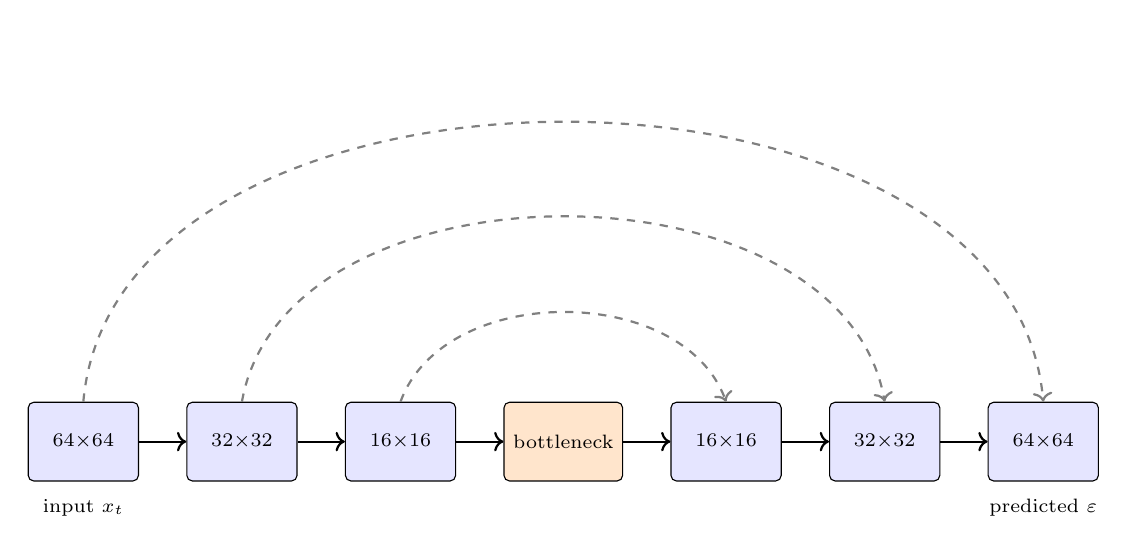
\begin{tikzpicture}[
    every node/.style={font=\scriptsize},
    block/.style={draw, rounded corners=2pt, minimum height=10mm, minimum width=14mm,
                  fill=blue!10},
    bneck/.style={draw, rounded corners=2pt, minimum height=10mm, minimum width=14mm,
                  fill=orange!20},
    skip/.style={->, dashed, gray, thick},
    arr/.style={->, thick},
]
  % Down path
  \node[block] (d1) {$64{\times}64$};
  \node[block, right=6mm of d1] (d2) {$32{\times}32$};
  \node[block, right=6mm of d2] (d3) {$16{\times}16$};
  \node[bneck, right=6mm of d3] (b)  {bottleneck};
  % Up path (mirror)
  \node[block, right=6mm of b]  (u3) {$16{\times}16$};
  \node[block, right=6mm of u3] (u2) {$32{\times}32$};
  \node[block, right=6mm of u2] (u1) {$64{\times}64$};
  % Forward arrows
  \draw[arr] (d1) -- (d2);
  \draw[arr] (d2) -- (d3);
  \draw[arr] (d3) -- (b);
  \draw[arr] (b)  -- (u3);
  \draw[arr] (u3) -- (u2);
  \draw[arr] (u2) -- (u1);
  % Skip connections (curve over the top)
  \draw[skip] (d3.north) to[out=70,in=110]  (u3.north);
  \draw[skip] (d2.north) to[out=80,in=100]  (u2.north);
  \draw[skip] (d1.north) to[out=85,in=95]   (u1.north);
  % Labels
  \node[below=1mm of d1] {input $\xT$};
  \node[below=1mm of u1] {predicted $\eps$};
\end{tikzpicture}
\caption{The U-Net at a glance. Down path compresses, the bottleneck holds
global context, the up path rebuilds, and skip connections (dashed) ferry
fine detail across.}
\end{figure}

\FloatBarrier

% -----------------------------------------------------------------------------
\subsection{Constructing the U-Net}
% -----------------------------------------------------------------------------

\begin{lstlisting}
unet = UNet2DModel(
    sample_size        = img_res,
    in_channels        = 1,
    out_channels       = 1,
    layers_per_block   = 2,
    block_out_channels = channel_width,
    down_block_types   = ("DownBlock2D",) * len(channel_width),
    up_block_types     = ("UpBlock2D",)   * len(channel_width),
    num_class_embeds   = num_classes + 1,   # +1 for the NULL class
).to(device)
unet = torch.nn.parallel.DistributedDataParallel(unet, device_ids=[local_rank])
\end{lstlisting}

\begin{description}[style=nextline,leftmargin=1.5em]
  \item[\code{sample\_size}] Spatial resolution the U-Net is built for.
        Inputs are $B \times 1 \times \text{img\_res} \times \text{img\_res}$.
  \item[\code{in\_channels / out\_channels}] EMNIST is greyscale, so $1$ in
        and $1$ out (predict noise of the same shape as the input).
  \item[\code{layers\_per\_block}] How many conv/resnet layers run inside
        each stage before moving to the next resolution.
  \item[\code{block\_out\_channels}] Channel widths at each U-Net stage; one
        entry per resolution level.
  \item[\code{down\_block\_types / up\_block\_types}] One block per stage;
        \code{DownBlock2D} halves the spatial size each stage, \code{UpBlock2D}
        doubles it. (We do \emph{not} use the attention variants --- probably
        overkill for EMNIST; worth testing.)
  \item[\code{num\_class\_embeds}] Size of the class-embedding table:
        \code{num\_classes + 1} (the extra slot is the \code{NULL\_CLASS}
        used for CFG dropout).
\end{description}

\code{DistributedDataParallel} wraps the model so each process uses its local
GPU and gradients are synced across ranks.

% -----------------------------------------------------------------------------
\subsection{The EMA model}
% -----------------------------------------------------------------------------

We create a second copy of the U-Net that does \emph{not} train directly.
After every optimizer step we update its weights using
\[
  w_{\text{ema}} \;\leftarrow\; \texttt{EMA\_DECAY}\cdot w_{\text{ema}}
                                 + (1 - \texttt{EMA\_DECAY}) \cdot w_{\text{current}}.
\]
So instead of jumping around like normal SGD updates, the EMA model changes
slowly and smoothly over time.

\paragraph{Why?} During training, model weights fluctuate from step to step;
some updates improve things, some slightly overshoot. The EMA version acts
like a smoothed version of the model across many recent training steps. In
diffusion models this almost always produces more stable generations, cleaner
samples, and better generalisation.

\paragraph{Important.} The optimizer updates the main U-Net.
The EMA U-Net is updated manually using the moving-average rule, lives in
\code{eval} mode, and has \code{requires\_grad\_(False)} on all of its
parameters --- it is never updated by gradients.

% -----------------------------------------------------------------------------
\subsection{Scheduler, optimizer, AMP}
% -----------------------------------------------------------------------------

\begin{lstlisting}
scheduler = DDPMScheduler(num_train_timesteps=STEPS, beta_schedule=BETA_SCHEDULE)
optimizer = torch.optim.AdamW(unet.parameters(), lr=LEARNING_RATE)
scaler    = torch.amp.GradScaler("cuda")
autocast_context = lambda: torch.amp.autocast("cuda", dtype=torch.float16)
\end{lstlisting}

\begin{description}[style=nextline,leftmargin=1.5em]
  \item[\code{DDPMScheduler}] Defines the forward diffusion process: how many
        timesteps and how the noise variance $\beta_t$ grows over time. Used
        to add noise to clean images during training.
  \item[\code{AdamW}] Standard optimiser for diffusion models.
  \item[\code{GradScaler} / \code{autocast}] When training in \code{float16},
        gradients can underflow. \code{GradScaler} dynamically scales the loss
        to keep training stable.
\end{description}

% =============================================================================
\section{The forward diffusion process}
% =============================================================================

In one forward diffusion step we define:
\[
  \eps_t \sim \mathcal{N}(0, I), \qquad \alpha_t = 1 - \beta_t,
\]
where $\beta_t$ is the fraction of \emph{new} noise injected at step $t$ and
$\alpha_t$ is the fraction of the \emph{previous} signal retained. Then
\[
  \boxed{\;\xT \;=\; \sqrt{\alpha_t}\,x_{t-1} \;+\; \sqrt{1-\alpha_t}\,\eps_t.\;}
\]

\paragraph{Why we do not loop step-by-step.} It may seem strange that each
batch contains images at different timesteps. In principle, an image at
timestep $T$ has received $T$ additions of Gaussian noise. But $T$ additions
of Gaussian noise with mean $M$ and variance $V$ is equivalent to one
addition of Gaussian noise with mean $T\,M$ and variance $T\,V$. With
$M=0$ and $V=1$, this simplifies to one addition of Gaussian noise with
mean $0$ and variance $T$.

In reality diffusion is slightly more complicated because we do \emph{not}
add the same amount of noise at every step. Instead, we use a noise schedule.
The default scheduler used here is \code{squaredcos\_cap\_v2}, which is a
cosine-based schedule. Intuitively, early timesteps add only a little noise,
and later timesteps add much more. This is usually better than noising too
aggressively at the start --- if we destroy the signal too quickly, then
later noising steps are less useful.

\paragraph{The closed form.} If we repeatedly apply the per-step rule from
$\xZero$ to $\xT$, we get the cumulative form
\[
  \xT \;=\; \sqrt{\abar_t}\,\xZero \;+\; \sqrt{1-\abar_t}\,\eps,
  \qquad
  \abar_t \;=\; \prod_{s=1}^{t}\alpha_s,
\]
where $\eps$ is a single Gaussian noise tensor representing the combined
effect of all the individual noise injections $\eps_1,\ldots,\eps_t$. This is
the key simplification that lets us compute $\xT$ in one shot, and it is
exactly what the scheduler does for us.

\begin{figure}[!htbp]
\centering
\vspace{4pt}
\resizebox{0.95\textwidth}{!}{%
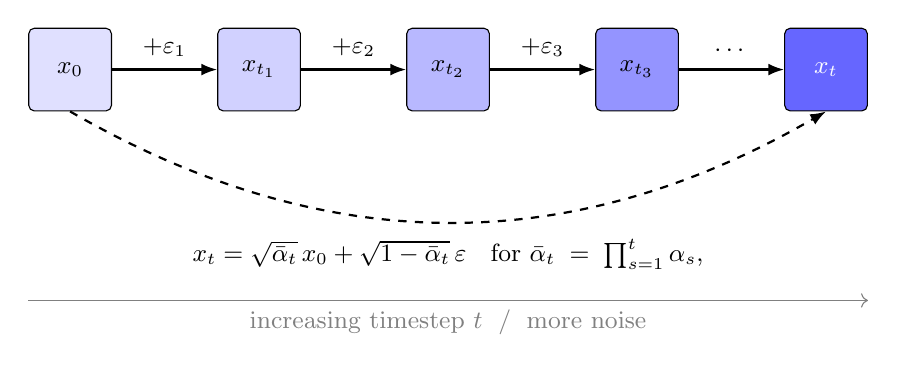
\begin{tikzpicture}[
  every node/.style={font=\small},
  img/.style={draw, rounded corners=2pt, minimum width=1.05cm,
              minimum height=1.05cm, align=center, inner sep=1pt},
  arr/.style={-{Latex[length=2mm]}, thick},
]
  % Five frames along a noise schedule: x0, x_{t1}, x_{t2}, x_{t3}, x_T
  \node[img, fill=blue!12] (x0)  at (0,0)   {$\xZero$};
  \node[img, fill=blue!18] (x1)  at (2.4,0) {$x_{t_1}$};
  \node[img, fill=blue!28] (x2)  at (4.8,0) {$x_{t_2}$};
  \node[img, fill=blue!42] (x3)  at (7.2,0) {$x_{t_3}$};
  \node[img, fill=blue!60, text=white] (xT) at (9.6,0) {$\xT$};

  % Per-step arrows with epsilon labels
  \draw[arr] (x0) -- node[above=1pt]{$+\eps_1$} (x1);
  \draw[arr] (x1) -- node[above=1pt]{$+\eps_2$} (x2);
  \draw[arr] (x2) -- node[above=1pt]{$+\eps_3$} (x3);
  \draw[arr] (x3) -- node[above=1pt]{$\cdots$} (xT);

  % Closed-form bypass arrow
  \draw[arr, dashed, bend right=30]
    (x0.south) to node[below=4pt, fill=white, inner sep=2pt]
      {\small $\xT = \sqrt{\abar_t}\,\xZero + \sqrt{1-\abar_t}\,\eps$ \; for $\abar_t \;=\; \prod_{s=1}^{t}\alpha_s,$}
    (xT.south);

  % Time axis
  \draw[->, gray] ($(x0.south west)+(0,-2.4)$) -- ($(xT.south east)+(0,-2.4)$)
    node[midway, below]{increasing timestep $t$ \;/\; more noise};
\end{tikzpicture}%
}
\caption{Forward diffusion as a Markov chain (solid arrows) versus the
closed-form jump (dashed arrow) that the scheduler actually uses. Each
solid step adds a fresh Gaussian noise tensor $\eps_i$ scaled by the noise
schedule; because sums of Gaussians are Gaussian, all $t$ steps collapse
into a single draw $\eps$ scaled by $\sqrt{1-\abar_t}$.}
\label{fig:forward-strip}
\end{figure}

\FloatBarrier
\bigskip

\noindent\textit{Reference for \code{squaredcos\_cap\_v2}:} Nichol \& Dhariwal,
\emph{Improved Denoising Diffusion Probabilistic Models} (2021),
\url{https://arxiv.org/abs/2102.09672}.

% =============================================================================
\section{Inside the training loop}
% =============================================================================

One epoch is one full pass through the entire dataset. The dataset is divided
into mini-batches; one mini-batch $\to$ one forward pass $\to$ one loss $\to$
one optimizer step.

\subsection{Setting up the epoch}

\begin{lstlisting}
for epoch in range(EPOCHS):
    sampler.set_epoch(epoch)        # synchronised reshuffle across GPUs
    t0 = time.time()
    if rank == 0 and tracker is not None:
        tracker.start_epoch()
    losses = []
\end{lstlisting}

The \code{DistributedSampler} reshuffles deterministically per epoch so each
GPU sees a different slice of the dataset, but in a synchronised way across
processes.

% -----------------------------------------------------------------------------
\subsection{One mini-batch, end to end}
% -----------------------------------------------------------------------------

The body of the inner loop is conceptually four steps:
\begin{enumerate}[leftmargin=*]
  \item Apply CFG dropout to the labels.
  \item Sample timesteps and noise; build $\xT$.
  \item Predict the noise with the U-Net; compute the MSE loss.
  \item Backprop with mixed precision; step the optimizer; update the EMA.
\end{enumerate}

% .............................................................................
\subsubsection{CFG dropout}
% .............................................................................

\begin{lstlisting}
dropout_mask = torch.rand(labels_batch.size(0), device=device) < CFG_DROPOUT_PROB
labels_cfg   = torch.where(
    dropout_mask,
    torch.full_like(labels_batch, NULL_CLASS),
    labels_batch,
)
\end{lstlisting}

\code{dropout\_mask} is a boolean vector like
\code{[False, True, False, False, True, ...]}. Wherever the mask is
\code{True}, the image is trained as if it were a member of the null class.
This is what allows us to do conditional/unconditional inference later --- it
is where our whole diffusion-geometry / force-zoo machinery comes from.

\begin{figure}[!htbp]
\centering
\vspace{4pt}
\resizebox{0.95\textwidth}{!}{%
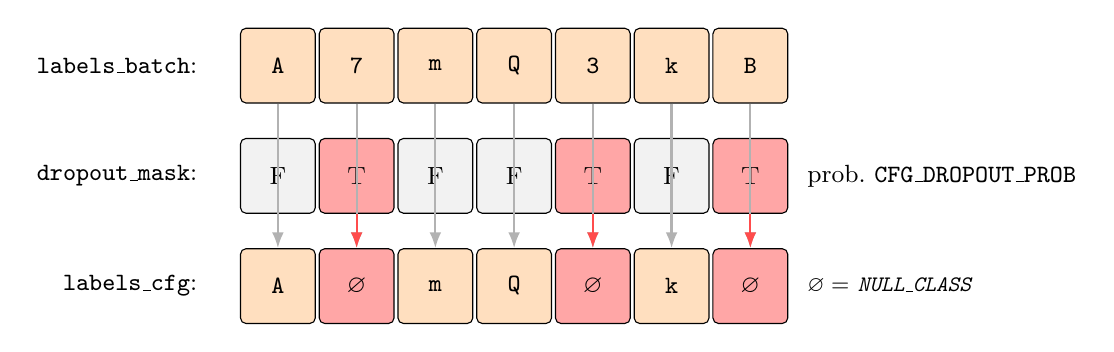
\begin{tikzpicture}[
  every node/.style={font=\small},
  cell/.style={draw, minimum width=0.95cm, minimum height=0.95cm,
               align=center, inner sep=1pt, rounded corners=2pt},
  arr/.style={-{Latex[length=2mm]}, thick},
]
  % Original labels row
  \node[anchor=east] at (-0.3,0) {\code{labels\_batch}:};
  \node[cell, fill=orange!25] (l1) at (0.6,0) {\texttt{A}};
  \node[cell, fill=orange!25] (l2) at (1.6,0) {\texttt{7}};
  \node[cell, fill=orange!25] (l3) at (2.6,0) {\texttt{m}};
  \node[cell, fill=orange!25] (l4) at (3.6,0) {\texttt{Q}};
  \node[cell, fill=orange!25] (l5) at (4.6,0) {\texttt{3}};
  \node[cell, fill=orange!25] (l6) at (5.6,0) {\texttt{k}};
  \node[cell, fill=orange!25] (l7) at (6.6,0) {\texttt{B}};

  % Dropout mask row
  \node[anchor=east] at (-0.3,-1.4) {\code{dropout\_mask}:};
  \node[cell, fill=gray!10]   (m1) at (0.6,-1.4) {F};
  \node[cell, fill=red!35]    (m2) at (1.6,-1.4) {T};
  \node[cell, fill=gray!10]   (m3) at (2.6,-1.4) {F};
  \node[cell, fill=gray!10]   (m4) at (3.6,-1.4) {F};
  \node[cell, fill=red!35]    (m5) at (4.6,-1.4) {T};
  \node[cell, fill=gray!10]   (m6) at (5.6,-1.4) {F};
  \node[cell, fill=red!35]    (m7) at (6.6,-1.4) {T};

  \node[anchor=west] at (7.2,-1.4)
    {prob.\ \code{CFG\_DROPOUT\_PROB}};

  % Output labels row (after torch.where)
  \node[anchor=east] at (-0.3,-2.8) {\code{labels\_cfg}:};
  \node[cell, fill=orange!25] (o1) at (0.6,-2.8) {\texttt{A}};
  \node[cell, fill=red!35]    (o2) at (1.6,-2.8) {$\varnothing$};
  \node[cell, fill=orange!25] (o3) at (2.6,-2.8) {\texttt{m}};
  \node[cell, fill=orange!25] (o4) at (3.6,-2.8) {\texttt{Q}};
  \node[cell, fill=red!35]    (o5) at (4.6,-2.8) {$\varnothing$};
  \node[cell, fill=orange!25] (o6) at (5.6,-2.8) {\texttt{k}};
  \node[cell, fill=red!35]    (o7) at (6.6,-2.8) {$\varnothing$};

  % Arrows from masked positions to null class
  \foreach \i in {1,...,7} {
    \draw[arr, gray!60] (l\i) -- (o\i);
  }
  % Highlight the dropped ones
  \draw[arr, red!70, thick] (m2.south) -- (o2.north);
  \draw[arr, red!70, thick] (m5.south) -- (o5.north);
  \draw[arr, red!70, thick] (m7.south) -- (o7.north);

  % Caption-ish annotation
  \node[anchor=west, font=\footnotesize\itshape] at (7.2,-2.8)
    {$\varnothing = $ \code{NULL\_CLASS}};
\end{tikzpicture}%
}
\caption{CFG dropout in one mini-batch. With probability
\code{CFG\_DROPOUT\_PROB} each label is replaced by the null class
$\varnothing$. The U-Net therefore sees a mixture of conditional and
unconditional examples in every batch, which is what makes
classifier-free guidance possible at inference time: the same network can
produce both $\eps_\theta(\xT, t, c)$ and $\eps_\theta(\xT, t, \varnothing)$.}
\label{fig:cfg-dropout}
\end{figure}

\FloatBarrier

% .............................................................................
\subsubsection{Sampling timesteps and noise}
% .............................................................................

\begin{lstlisting}
timesteps_batch = torch.randint(low=0, high=STEPS,
                                size=(images_batch.size(0),), device=device)
noise_batch     = torch.randn_like(images_batch)
noisy_images_batch = scheduler.add_noise(
    original_samples = images_batch,    # x_0
    noise            = noise_batch,     # epsilon
    timesteps        = timesteps_batch, # t (per image)
)
\end{lstlisting}

\paragraph{Why random timesteps?} The model must learn to denoise images at
\emph{every possible noise level}. Looping over all timesteps sequentially
would be inefficient, so for each image we sample a timestep uniformly:
\[
  \mathbb{E}_t\bigl[\mathrm{MSE}(\eps_{\text{pred}}, \eps)\bigr]
\]
is approximated by averaging over many random $(t, \xT, \eps)$ triplets.
Within a single mini-batch some images are lightly corrupted, some
moderately, and some heavily; over many mini-batches this random sampling
approximates the full expectation.

% .............................................................................
\subsubsection{Forward pass and loss}
% .............................................................................

\begin{lstlisting}
optimizer.zero_grad(set_to_none=True)
with autocast_context():
    predicted_noise_batch = unet(
        noisy_images_batch,
        timesteps_batch,
        class_labels=labels_cfg,
    ).sample
    loss = F.mse_loss(predicted_noise_batch, noise_batch)
\end{lstlisting}

The U-Net is trained to solve: \emph{``Given $\xT$ (the clean image with $t$
additions of Gaussian noise), can you recover the exact noise $\eps$ that was
added?''}

Why predict noise instead of the clean image directly?
\begin{itemize}
  \item The noise distribution is simple (Gaussian), making it easier to learn.
  \item The same objective works across all timesteps.
  \item Empirically this gives more stable training and better results.
\end{itemize}

The output \code{predicted\_noise\_batch} has the same shape as the input.
The MSE is averaged across all pixels, channels, and images in the
mini-batch, producing a single scalar that answers ``how wrong was the model
on this entire mini-batch?''.

% .............................................................................
\subsubsection{Backprop with mixed precision and the optimizer step}
% .............................................................................

\begin{lstlisting}
scaler.scale(loss).backward()     # compute gradients (scaled)
scaler.unscale_(optimizer)        # unscale for accurate norms / clipping
grad_norm_val = compute_grad_norm(unet.module)
scaler.step(optimizer)            # update the live UNet
scaler.update()                   # adjust scaling factor for next step
\end{lstlisting}

We trained inside an \code{autocast} \code{float16} context, which improves
speed and reduces memory usage but can cause gradients to underflow.
\code{GradScaler}:
\begin{enumerate}
  \item scales the loss upward before \code{backward()},
  \item unscales gradients before the optimizer step, and
  \item dynamically adjusts its scaling factor over time.
\end{enumerate}
This is what makes mixed-precision training stable.

% .............................................................................
\subsubsection{EMA update}
% .............................................................................

\begin{lstlisting}
with torch.no_grad():
    for ema_param, current_param in zip(ema_unet.parameters(),
                                        unet.module.parameters()):
        ema_param.mul_(EMA_DECAY).add_(current_param, alpha=1 - EMA_DECAY)
\end{lstlisting}

For each parameter,
\[
  w_{\text{ema}} \;\leftarrow\;
  \texttt{EMA\_DECAY}\cdot w_{\text{ema}} +
  (1 - \texttt{EMA\_DECAY}) \cdot w_{\text{current}}.
\]
\code{EMA\_DECAY} is typically close to $1$ (e.g.\ $0.999$), so the EMA model
changes slowly and represents a long-term average of recent weights. The
optimizer updates the live U-Net; the EMA U-Net is never touched by
gradients.

% -----------------------------------------------------------------------------
\subsection{End of epoch: logging and checkpointing}
% -----------------------------------------------------------------------------

After all mini-batches:
\begin{itemize}
  \item Compute mean mini-batch loss across the epoch (a rough training signal,
        not a validation metric).
  \item Compute elapsed time \code{dt = time.time() - t0}.
  \item Only \textbf{rank 0} logs and saves; in distributed training every GPU
        runs this script and we restrict logging/checkpointing to avoid
        duplication.
  \item Write an EMA checkpoint to
        \code{checkpoints/SIZE\_NAME/emnist\_MODEL\_NAME\_epochNNN.pt}
        containing the EMA \code{state\_dict}, the class list, the scheduler
        config, image size, channel widths, the variation name, the epoch,
        the dataset split, beta schedule, EMA decay, CFG dropout probability,
        the null-class index, and \code{num\_class\_embeds}.
\end{itemize}

% =============================================================================
\section{Post-training: plots, report, clean shutdown}
% =============================================================================

When training finishes (rank 0 only):

\begin{enumerate}[leftmargin=*]
  \item \code{generate\_all\_plots(tracker)} writes plots to
        \code{metrics/output/SIZE\_NAME/plots}.
  \item \code{generate\_report(tracker, config=TRAINING\_CONFIG, plot\_paths=\dots)}
        writes a Markdown report alongside them.
  \item Both CSV and JSON metric files (\code{tracker.csv\_path},
        \code{tracker.json\_path}) are also retained.
\end{enumerate}

Finally we tear down the distributed group:
\begin{lstlisting}
torch.distributed.destroy_process_group()
\end{lstlisting}

\medskip
\noindent\textbf{Summary.} \code{train.py} stitches together a small number of
moving parts --- \code{UNet2DModel}, \code{DDPMScheduler}, AdamW, EMA, AMP,
CFG dropout, distributed sampling --- into a single training loop whose only
job is to learn $\eps_{\text{pred}} = f(\xT, t, \texttt{class\_label})$. Once
that function is learned, the EMA checkpoints become the input to everything
else in this repo.

\end{document}
